\subsection{Arquitectura del Process-Component}

El Process-Component es un proyecto independiente a LUCA y que deberá de ser implementado. Su objetivo es fundamentalmente ejercer las labores de la vista, y se in componente encargado de mostrar elementos en pantalla.

La arquitectura del Process-Component se ostenta en dos pilares. El primero la lógica de negocio del propio componente y el segundo es un fichero conector que se comunica con una librería de \emph{GO.JS} que también debe de ser definida.

Este componente se compone de un modelo de datos que deberá de ser implementado por cualquier proyecto que quiera usarlo. Su principal característica es poseer un conjunto de métodos encargados de crear, modificar y eliminar los diferentes elementos que serán plasmados en la vista. Este modelo será traducido a un conjunto de clases diseñadas específicamente para ser enviadas al \emph{Conector} para que este visualice los datos.


El \emph{Conector} internamente importa la librería gráfica \emph{GoJS} (será explicada en apartados posteriores) y se encargará insertar, modificar o eliminar los elementos del modelo de esta librería. Por lo tanto actuará de intermediario entre el modelo del \emph{Process-Component} y de \emph{GoJS}.

A continuación, se muestra una figura explicativa de dicha interacción interna entre los componentes:

\begin{figure}[!tb]
	\centering
	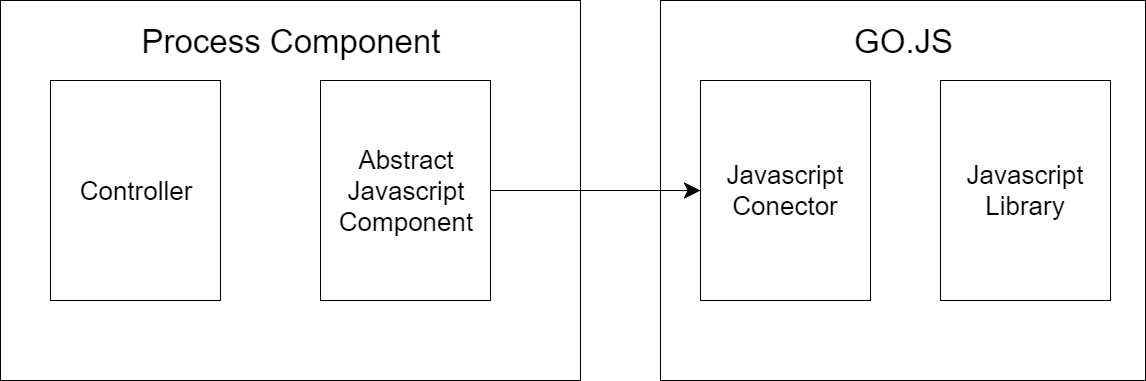
\includegraphics[width=\linewidth]{processComponentArquitectura.png}
	\caption{Arquitectura del Process-Component}\label{fig:processComponent}
\end{figure}

Como resumen del funcionamiento del Process-Component, éste es el encargado de recibir eventos realizados sobre la interfaz gráfica, a través del conector hasta llegar a la lógica del componente donde se tratarán y de realizar modificaciones sobre la vista.


\subsection{Pruebas}
	
	
	Las pruebas se centraron principalmente en el Luca-Process, ya que es el componente que alberga la mayor lógica del proyecto debido al conjunto de servicios que lo compone y a la lógica de negocio que incorpora.
	
	
	Profundizando en las pruebas implementadas, solo se han realizado pruebas de integración por varios motivos. El primero es que las pruebas unitarias no son necesarias hacerlas ya que se centran sobre la capa de repositorio y esta capa ha sido implementada con Spring Data Jpa\cite{jpa}, este framework ofrece una comunicación con la base de datos fiable y ya ha sido probada y certificada por otros organismos, por lo tanto, no es necesario realizar pruebas de su funcionamiento. El motivo por el que no se realizaron pruebas de sistema, aunque en una primera planificación estaban previstas hacerlas integrándolas con Selenium\cite{selenium} fue la complejidad que lleva la integración junto con Vaadin\cite{vaadin}, ya que la ventaja de programar mediante una captura de eventos sobre la vista toda la secuencia de movimiento sobre dicha vista pasa a ser programática, y debido a que había que ceñirse a unas fechas de entrega y al tiempo que llevaría dicha implementación se decidió omitirlas.

	
	Las pruebas de integración que se llevaron a cabo se implementaron con Spring Test\cite{springTest} y JUnit\cite{junit}. Cada test ejecutado se compone de un fichero \emph{SQL} que cargará datos en la base de datos (en nuestro caso se utilizó una base de datos relacional) durante la ejecución, es decir, una vez finalizado el test la base de datos vuelve a su estado original, de esta forma se pueden hacer consultas a la misma sin alterar su estado para siguientes tests. Se ejecutaron pruebas sobre las acciones \emph{CRUD}\cite{crud} de cada servicio, además, se hicieron las pruebas también sobre un objeto que actúa como \emph{DTO}\cite{dto} que contiene el estado del proceso, de forma que se ha comprobado que las operaciones \emph{CRUD} sobre este objeto funciona (por ejemplo el guardado de un proceso con todos sus elementos que lo acompañan).



